\subsection{Blockchain Fundamentals}

Instead of keeping records on one central machine, blockchain splits that data up across a whole network of computers using distributed ledger technology. Since everyone on the network holds their own exact copy of this ledger, going back and secretly changing or faking a record is incredibly hard without getting the whole network to agree on the change. This unique focus on security explains why blockchain keeps getting picked up for real-world setups in banking, tracking supply chains, digital identity, and even IoT tech\cite{zheng2017blockchain}.

You can essentially picture a blockchain as a shared public record books. Transactions get grouped together into individual blocks, and this chain just keeps growing longer as new blocks get tacked onto the end of it over time. To make sure everything stays accurate and nobody can tamper with the data, the network relies on a mix of asymmetric cryptography and distributed consensus algorithms. When people talk about blockchain's main strengths, they usually point to things like decentralization, permanent records, user anonymity, and audit trails. These exact features are what help companies cut down on extra costs and make verification processes run a whole lot faster.

\subsubsection{Decentralization}
Most traditional computer setups use an old-school client-server model. In that setup, one company or database manager holds all the keys to the data. That administrator or any user with special rights can easily hop into the database and change things. This setup opens the door to major risks like a single point of failure (SPoF)\cite{yuan2014testing} or internal data fraud. Decentralized networks fix this vulnerability by switching over to a Peer-to-Peer (P2P) setup instead. In a P2P layout, computers talk straight to each other instead of routing everything through a central server\cite{stoica_chord}. Every single computer acts as both a client and a server at the same time, saving its own live copy of the entire ledger. Because of this layout, no single user can log in and rewrite history from their own computer. If you want to change the system state or add new entries, a strict majority of the network has to approve it first. We will break down exactly how this voting process works in Section 2.1.4.

\begin{figure}[H]
    \centering
    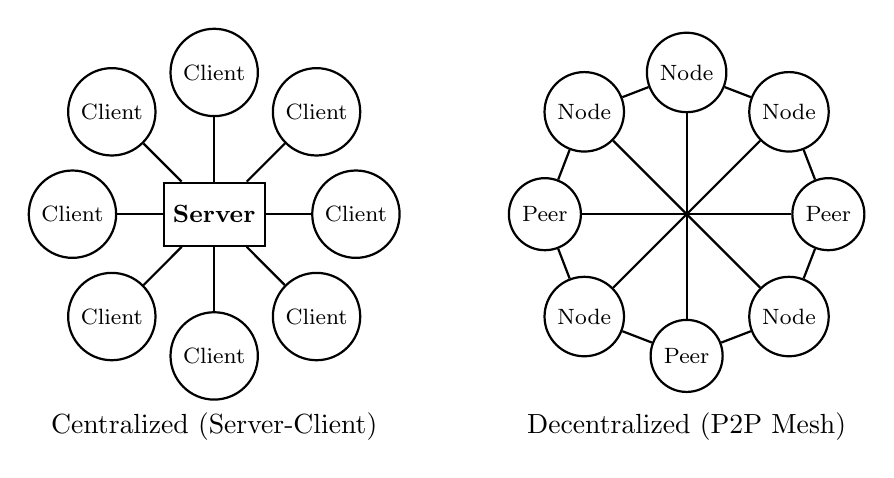
\begin{tikzpicture}[
        clientNode/.style={
            circle,
            draw,
            thick,
            minimum size=0.8cm,
            font=\footnotesize
        },
        serverNode/.style={
            rectangle,
            draw,
            thick,
            minimum size=0.8cm,
            font=\small\bfseries
        },
        line/.style={
            thick
        }
    ]
        \node[serverNode] (server) at (0,2) {Server};
        
        \node[clientNode] (c1) at (0,3.8)  {Client};
        \node[clientNode] (c2) at (1.3,3.3) {Client};
        \node[clientNode] (c3) at (1.8,2)   {Client};
        \node[clientNode] (c4) at (1.3,0.7) {Client};
        \node[clientNode] (c5) at (0,0.2)  {Client};
        \node[clientNode] (c6) at (-1.3,0.7){Client};
        \node[clientNode] (c7) at (-1.8,2)  {Client};
        \node[clientNode] (c8) at (-1.3,3.3){Client};
        
        \draw[line] (server) -- (c1);
        \draw[line] (server) -- (c2);
        \draw[line] (server) -- (c3);
        \draw[line] (server) -- (c4);
        \draw[line] (server) -- (c5);
        \draw[line] (server) -- (c6);
        \draw[line] (server) -- (c7);
        \draw[line] (server) -- (c8);
        
        \node[anchor=north, yshift=-0.4cm] at (0,0) {Centralized (Server-Client)};

        \node[clientNode] (p1) at (6,3.8)  {Node};
        \node[clientNode] (p2) at (7.3,3.3) {Node};
        \node[clientNode] (p3) at (7.8,2)   {Peer};
        \node[clientNode] (p4) at (7.3,0.7) {Node};
        \node[clientNode] (p5) at (6,0.2)  {Peer};
        \node[clientNode] (p6) at (4.7,0.7) {Node};
        \node[clientNode] (p7) at (4.2,2)   {Peer};
        \node[clientNode] (p8) at (4.7,3.3) {Node};
        
        \draw[line] (p1) -- (p2);
        \draw[line] (p2) -- (p3);
        \draw[line] (p3) -- (p4);
        \draw[line] (p4) -- (p5);
        \draw[line] (p5) -- (p6);
        \draw[line] (p6) -- (p7);
        \draw[line] (p7) -- (p8);
        \draw[line] (p8) -- (p1);

        \draw[line] (p1) -- (p5);
        \draw[line] (p3) -- (p7);
        \draw[line] (p2) -- (p6);
        \draw[line] (p4) -- (p8);
        
        \node[anchor=north, yshift=-0.4cm] at (6,0) {Decentralized (P2P Mesh)};

    \end{tikzpicture}
    \vspace{0.3cm}
    \caption{Centralized (Server-Client) and Decentralized (Peer-to-Peer) network}
    \label{fig:comparison_topologies}
\end{figure}

\subsubsection{Blocks}
A block is really just a data packet used to gather a bunch of transactions or updates together at once. Instead of updating a database line by line, the system bundles records chronologically to make verifying them much easier. Every single block comes with two main pieces: a body and a header. The block body is where the actual transactions sit, along with a counter telling you how many are inside. The total amount of data you can cram into a single block depends entirely on the block size limit and how large each individual transaction happens to be\cite{zheng2017blockchain}. Over in the block header, you will find these specific tracking details:

\begin{itemize}
    \item Block version: A basic marker showing which exact set of software validation rules the network needs to follow for this block\cite{zheng2017blockchain}.

    \item Merkle tree root hash: This is a single cryptographic code that represents the combined fingerprint of every single transaction packed inside that block\cite{zheng2017blockchain}.

    \item Timestamp: Shows the exact moment the block was created, recorded in seconds since the standard start date of January 1, 1970\cite{zheng2017blockchain}.

    \item nBits: A target number that sets how hard it is to calculate a valid hash for the block\cite{zheng2017blockchain}.

    \item Nonce: A small 4-byte counter variable. It starts off at 0 and ticks up by one every single time the system runs a new hash calculation (more on this in Section III)\cite{zheng2017blockchain}.

    \item Previous block hash: A 256-bit cryptographic signature that points straight back to the block right before it, which is what actually locks the chain together\cite{zheng2017blockchain}.
\end{itemize}

\begin{figure}[H]
    \centering
    
    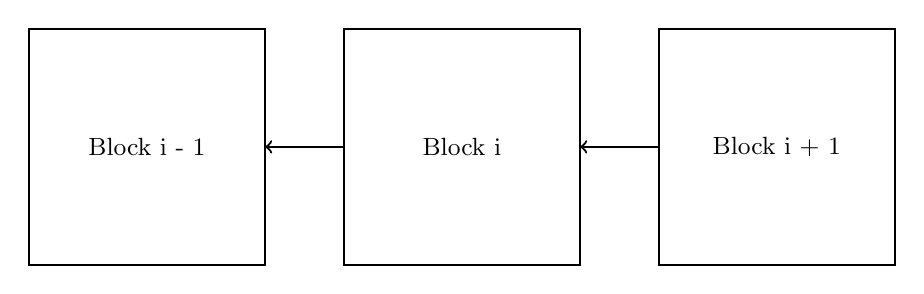
\begin{tikzpicture}[
        node distance=2cm,
        every node/.style={
            font=\small 
        }
    ]
        % Block 1
        \begin{scope}[xshift=0cm]
            \draw[thick] (0, 0) rectangle (3, 3);

            \node at (1.5, 1.5) {Block i - 1};
        \end{scope}

        % Block 2
        \begin{scope}[xshift=4cm]
            \draw[thick] (0, 0) rectangle (3, 3);

            \node at (1.5, 1.5) {Block i};
        \end{scope}

        % Block 3
        \begin{scope}[xshift=8cm]
            \draw[thick] (0, 0) rectangle (3, 3);

            \node at (1.5, 1.5) {Block i + 1};
        \end{scope}

        \draw[<-, thick] (3,1.5) -- (4,1.5);

        \draw[<-, thick] (7,1.5) -- (8,1.5);
        
    \end{tikzpicture}
    
    \caption{Blockchain architecture}
    
    \label{fig:blockchain_architecture}
\end{figure}

\begin{figure}[H]
    \centering
    
    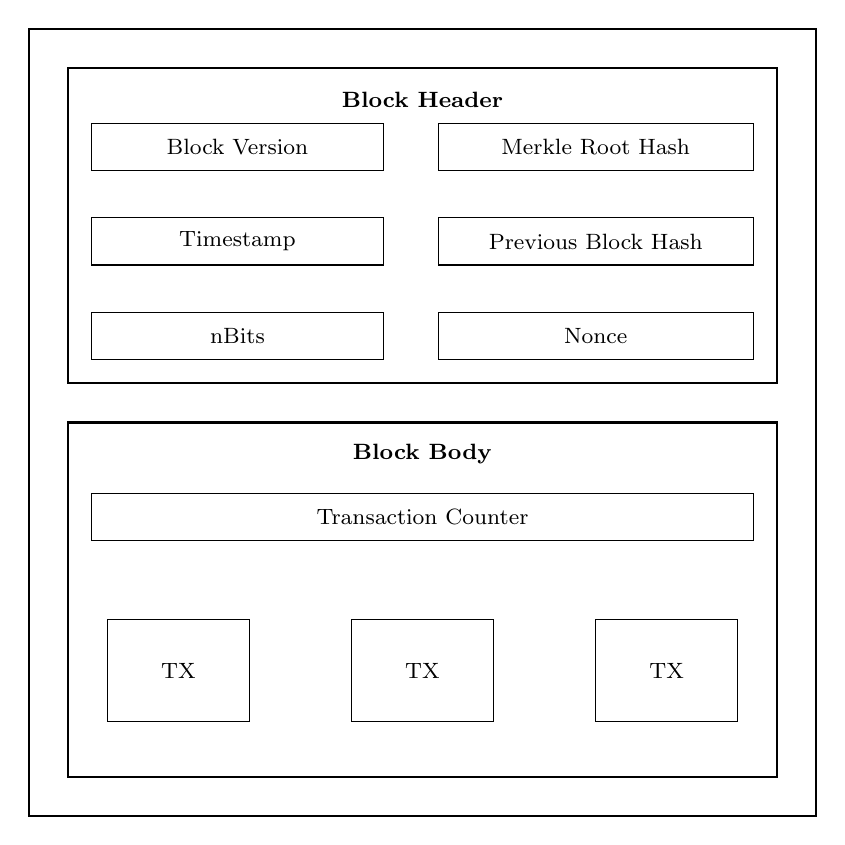
\begin{tikzpicture}[
        node distance=2cm,
        every node/.style={
            font=\footnotesize
        }
    ]
        % Block 1
        \begin{scope}[xshift=0cm]
            \draw[thick] (0,0) rectangle (10,10);
            
            % HEADER 
            \draw[thick] (0.5,5.5) rectangle (9.5,9.5);
            
            \node at (5,9.1) {\textbf{Block Header}};
            
            \draw (0.8,8.2) rectangle (4.5,8.8);
            \node at (2.65,8.5) {Block Version};
            
            \draw (5.2,8.2) rectangle (9.2,8.8);
            \node at (7.2,8.5) {Merkle Root Hash};
            
            \draw (0.8,7.0) rectangle (4.5,7.6);
            \node at (2.65,7.3) {Timestamp};
            
            \draw (5.2,7.0) rectangle (9.2,7.6);
            \node at (7.2,7.3) {Previous Block Hash};
            
            \draw (0.8,5.8) rectangle (4.5,6.4);
            \node at (2.65,6.1) {nBits};
            
            \draw (5.2,5.8) rectangle (9.2,6.4);
            \node at (7.2,6.1) {Nonce};
            
            % BODY 
            \draw[thick] (0.5,0.5) rectangle (9.5,5);
            
            \node at (5,4.6) {\textbf{Block Body}};
            
            \draw (0.8,3.5) rectangle (9.2,4.1);
            \node at (5,3.8) {Transaction Counter};
            
            \draw (1,1.2) rectangle (2.8,2.5);
            \node at (1.9,1.85) {TX};
            
            \draw (4.1,1.2) rectangle (5.9,2.5);
            \node at (5,1.85) {TX};
            
            \draw (7.2,1.2) rectangle (9,2.5);
            \node at (8.1,1.85) {TX};
        \end{scope}
    \end{tikzpicture}
    
    \caption{A block properties}
    
    \label{fig:block_properties}
\end{figure}

\subsubsection{Hashing}
Hashing is just a method where you pass any kind of input data through a math formula to spit out a fixed-length text string\cite{yaga2018blockchain}. The moment you run plain text or a file through a hash function, you get a completely unique digital code. Bitcoin and a lot of other big blockchain systems use an algorithm called SHA-256\cite{wikipedia_bitcoin}. It does not matter how big or small your input file is; SHA-256 takes that data and turns it into a standard 256-bit code. The math behind it is incredibly intense, making it practically impossible for regular computers to reverse the hash and figure out what the original file looked like. That said, down the road, breakthroughs in quantum computing might end up threatening the security of these current hashing styles.

\subsubsection{Consensus}
A consensus mechanism is basically a group protocol used to get an entire network of separate, untrusted computers to agree on one single version of the truth. It completely solves tricky issues like "double-spending" or entering duplicate data entries without needing a boss or a central company to watch over everyone\cite{morel2023bitcoin}.

While developers have come up with several ways to handle consensus—like Proof-of-Work (PoW), Proof-of-Concept (PoC), Proof-of-Stake (PoS), and various mashup models\cite{nguyen2019pos}—the two setups you see used the most are PoW and PoS.

\begin{itemize}
    \item Proof-of-Work: Network miners grab pending transactions out of a temporary memory pool (mempool) and piece together candidate blocks. Every candidate block is essentially a draft of what could become the next link in the chain. Miners then run a loop where they change a number called a nonce and run the block header through SHA-256 over and over again. They keep doing this until they get a final hash value that drops below the network's current difficulty target\cite{nakamoto2008bitcoin}. The moment a miner hits a winning hash, they blast the block out to the rest of the network. Full nodes then double-check the math on their own, and if it looks good, they add it to their personal copy of the chain.

          \begin{figure}[H]
    \centering
    
    \resizebox{\textwidth}{!}{
        \begin{tikzpicture}[
            every node/.style={font=\footnotesize},
            stepbox/.style={rectangle, draw, thick, text width=2.4cm, align=center, minimum height=1.5cm, rounded corners=3pt, fill=gray!5},
            descbox/.style={text width=2.4cm, align=left, font=\scriptsize, inner sep=2pt},
            container/.style={rectangle, draw, dashed, thick, rounded corners=5pt, inner sep=10pt},
            arrow/.style={-Stealth, thick, draw=black},
            blocknode/.style={rectangle, draw, thick, minimum size=0.5cm}
        ]

            \node (s1) [stepbox] {\textbf{1. Collect Transactions}};
            \node (d1) [descbox, below=0.1cm of s1] {Miners collect unconfirmed transactions from the mempool.};
            
            \node (s2) [stepbox, right=0.5cm of s1] {\textbf{Construct Candidate Block}};
            \node (d2) [descbox, below=0.1cm of s2] {Miner builds a candidate block with transactions and block header.};
            
            \node (s3) [stepbox, right=0.5cm of s2] {\textbf{Test Different Nonce Values}};
            \node (d3) [descbox, below=0.1cm of s3] {Miner repeatedly changes the nonce value.};
            
            \node (s4) [stepbox, right=0.5cm of s3] {\textbf{Hash the Block Header}};
            \node (d4) [descbox, below=0.1cm of s4] {The block header is hashed twice using SHA-256.};
            
            \node (s5) [diamond, draw, aspect=1.3, thick, text width=1.5cm, align=center, right=0.5cm of s4, inner sep=0pt] {\textbf{Hash $<=$ Target?}};
            \node (d5) [descbox, below=0.1cm of s5] {Check if the hash is smaller than the current PoW target.};
            
            \node (s6) [stepbox, right=0.6cm of s5] {\textbf{Valid block found}};
            \node (d6) [descbox, below=0.1cm of s6] {If valid, the miner has found a valid block};
    
            \draw [arrow] (s1) -- (s2);
            \draw [arrow] (s2) -- (s3);
            \draw [arrow] (s3) -- (s4);
            \draw [arrow] (s4) -- (s5);
            \draw [arrow] (s5) -- node[above, font=\scriptsize\bfseries] {Yes} (s6);
            \draw [arrow] (s5.north) -- ++(0,0.5) node[right, font=\scriptsize\bfseries] {No} -| (s3.north);
    
            \node (s7) [stepbox, fill=gray!2, text width=5cm, below=2.5cm of s3.south east] {\textbf{Broadcast to the Network}};
            \node (d7) [text width=5cm, align=left, font=\scriptsize, right=0.2cm of s7] {The valid block is broadcast to all nodes in the network.};
            
            \draw [arrow] (s6.south) |- (s7.east);
    
            \node (n1) [rectangle, draw, rounded corners=1pt, fill=white, text width=2.2cm, below=2cm of s7.south west, xshift=-1cm] {
                \textbf{Node 1}\\
                $\square$ Verify block header\\
                $\square$ Verify transactions\\
                $\square$ Verify Merkle root\\
                $\square$ Verify PoW
            };
            
            \node (n2) [rectangle, draw, rounded corners=1pt, fill=white, text width=2.2cm, right=0.3cm of n1] {
                \textbf{Node 2}\\
                $\square$ Verify block header\\
                $\square$ Verify transactions\\
                $\square$ Verify Merkle root\\
                $\square$ Verify PoW
            };
            
            \node (dots) [right=0.3cm of n2, font=\large\bfseries] {...};
            
            \node (nn) [rectangle, draw, rounded corners=1pt, text width=2.2cm, right=0.3cm of dots] {
                \textbf{Node 3}\\
                $\square$ Verify block header\\
                $\square$ Verify transactions\\
                $\square$ Verify Merkle root\\
                $\square$ Verify PoW
            };
            
            \node (s8_container) [container, fit=(n1) (n2) (dots) (nn)] {};
            \node[draw, thick, rounded corners=2pt, font=\small\bfseries, above=0pt of s8_container.north] {Full Nodes Independently Validate the Block};
            
            \draw [arrow] (s7.south) -- (s8_container.north);

            \node (s9) [rectangle, draw, thick, rounded corners=3pt, text width=6cm, align=center, minimum height=0.8cm, below=1.2cm of s8_container] {\textbf{Block Added to the Blockchain}};
            \node (d9) [text width=5cm, align=left, font=\scriptsize, right=0.3cm of s9] {Once the block is accepted by the network, it becomes the next official block.};
            
            \draw [arrow] (s8_container.south) -- (s9.north);
    
            \node (s10_title) [font=\small\bfseries, below=1.8cm of s9, xshift=-2.5cm] {Edge case: Longest Chain rule};
            
            \coordinate (chainorigin) at ($(s10_title.south) + (-2.5cm, -0.8cm)$);
            
            \node (b1) [blocknode] at (chainorigin) {};
            \node (b2) [blocknode, right=0.6cm of b1] {};
            \draw [arrow] (b1) -- (b2);
            
            \node (b3_top) [blocknode, right=0.8cm of b2, yshift=0.6cm] {};
            \node (b4_top) [blocknode, right=0.6cm of b3_top, fill=gray!40] {};
            \node (b5_top) [blocknode, right=0.6cm of b4_top, fill=gray!80] {};
            
            \draw [arrow] (b2) |- (b3_top);
            \draw [arrow] (b3_top) -- (b4_top);
            \draw [arrow] (b4_top) -- (b5_top);
            \node (label_top) [right=0.2cm of b5_top, font=\scriptsize\bfseries] {Chain A: Longest Chain (Accepted)};
            
            \node (b3_bot) [blocknode, right=0.8cm of b2, yshift=-0.6cm] {};
            \node (b4_bot) [blocknode, right=0.6cm of b3_bot] {};
            
            \draw [arrow] (b2) |- (b3_bot);
            \draw [arrow] (b3_bot) -- (b4_bot);
            \node (label_bot) [right=0.2cm of b4_bot, font=\scriptsize, color=gray!90] {Chain B: Orphan Chain (Rejected)};
    
        \end{tikzpicture}
    }
    
    \caption{Proof-of-Work workflow}
    \label{fig:pow_workflow}
\end{figure}

    \item Proof-of-Stake: This setup was built specifically to get around the massive electricity bills and heavy computing power that mining demands. Instead of having computers race each other to solve math puzzles, PoS handpicks block creators (called validators). The system chooses them based on things like how many network coins they have locked up as a deposit, mixed with a bit of random luck\cite{buterin2019casper}. The chosen validator compiles the next block on their own. From there, other network validators check the work, and if they agree it is valid, the block gets officially stamped into the blockchain ledger\cite{nguyen2019pos}\cite{buterin2019casper}.

          \begin{figure}[H]
    \centering
    \resizebox{\textwidth}{!}{
        \begin{tikzpicture}[
                every node/.style={font=\footnotesize},
                stepbox/.style={rectangle, draw, thick, text width=2.4cm, align=center, minimum height=1.5cm, rounded corners=3pt, fill=gray!5},
                descbox/.style={text width=2.4cm, align=left, font=\scriptsize, inner sep=2pt},
                container/.style={rectangle, draw, dashed, thick, rounded corners=5pt, inner sep=10pt},
                arrow/.style={-Stealth, thick, draw=black},
                actionnode/.style={rectangle, draw, thick, minimum height=0.6cm, rounded corners=2pt, fill=white}
            ]

            \node (s1) [stepbox] {\textbf{Stake Tokens \& Become Validator}};
            \node (d1) [descbox, below=0.1cm of s1] {Participants stake cryptocurrency to become validators};
            
            \node (s2) [stepbox, right=0.5cm of s1] {\textbf{Select block proposer}};
            \node (d2) [descbox, below=0.1cm of s2] {Validator selection depends on randomized selection and stake size};
            
            \node (s3) [stepbox, right=0.5cm of s2] {\textbf{Construct candidate block}};
            \node (d3) [descbox, below=0.1cm of s3] {The chosen validator bundles pending transactions into a candidate block};
            
            \node (s4) [stepbox, right=0.5cm of s3] {\textbf{Validate the candidate block}};
            \node (d4) [descbox, below=0.1cm of s4] {Other validators are randomly selected to validate the candidate block};
            
            \node (s5) [diamond, draw, aspect=1.3, thick, text width=1.5cm, align=center, right=0.5cm of s4, inner sep=0pt] {\textbf{>2/3 Validators agree?}};
            \node (d5) [descbox, below=0.1cm of s5] {Check if a supermajority of validators approve the block};
            
            \node (s6) [stepbox, right=0.6cm of s5] {\textbf{Block finalized}};
            \node (d6) [descbox, below=0.1cm of s6] {If approved, the network reaches consensus on the candidate block};

            \draw [arrow] (s1) -- (s2);
            \draw [arrow] (s2) -- (s3);
            \draw [arrow] (s3) -- (s4);
            \draw [arrow] (s4) -- (s5);
            \draw [arrow] (s5) -- node[above, font=\scriptsize\bfseries] {Yes} (s6);
            \draw [arrow] (s5.north) -- ++(0,0.5) node[right, font=\scriptsize\bfseries] {No} -| (s2.north);

            \node (s7) [stepbox, fill=gray!2, text width=5cm, below=2.5cm of s3.south east] {\textbf{Broadcast to the Network}};
            \node (d7) [text width=5cm, align=left, font=\scriptsize, right=0.2cm of s7] {The approved block is broadcast to the network};
            
            \draw [arrow] (s6.south) |- (s7.east);

            \node (n1) [rectangle, draw, rounded corners=2pt, text width=2.2cm, below=2cm of s7.south west, xshift=-1cm] {
                \textbf{Node 1}\\
                $\square$ Update blockchain state\\
                $\square$ Store finalized block\\
            };
            
            \node (n2) [rectangle, draw, rounded corners=2pt, text width=2.2cm, right=0.3cm of n1] {
                \textbf{Node 2}\\
                $\square$ Update blockchain state\\
                $\square$ Store finalized block\\
            };
            
            \node (dots) [right=0.3cm of n2, font=\large\bfseries] {...};
            
            \node (nn) [rectangle, draw, rounded corners=2pt, text width=2.2cm, right=0.3cm of dots] {
                \textbf{Node N}\\
                $\square$ Update blockchain state\\
                $\square$ Store finalized block\\
            };
            
            \node (s8_container) [container, fit=(n1) (n2) (dots) (nn)] {};
            \node[draw, thick, rounded corners=2pt, font=\small\bfseries, above=0pt of s8_container.north] {Full nodes update blockchain state};
            
            \draw [arrow] (s7.south) -- (s8_container.north);

            \node (s9_title) [font=\small\bfseries, below=1.8cm of s8_container, xshift=-2.0cm] {Edge case: Incentive Distribution \& Slashing Resolution};
            
            \node (b1) [actionnode, below=0.8cm of s9_title, xshift=-3.5cm] {\textbf{Validator evaluation}};
            
            \node (b3_top) [actionnode, right=1.0cm of b1, yshift=0.6cm, fill=gray!15] {\textbf{Honest Validator}};
            \node (b4_top) [rectangle, draw, right=0.5cm of b3_top, font=\scriptsize] {Earn Staking Rewards + Tx Fees};
            \draw [arrow] (b1) |- (b3_top);
            \draw [arrow] (b3_top) -- (b4_top);
            \node (label_top) [right=0.2cm of b4_top, font=\scriptsize\bfseries] {(Validator Stake Returned/Maintained)};
            
            \node (b3_bot) [actionnode, right=1.0cm of b1, yshift=-0.6cm, fill=gray!40] {\textbf{Malicious Validator}};
            \node (b4_bot) [rectangle, draw, right=0.5cm of b3_bot, font=\scriptsize] {Slashing Event Activated};
            \draw [arrow] (b1) |- (b3_bot);
            \draw [arrow] (b3_bot) -- (b4_bot);
            \node (label_bot) [right=0.2cm of b4_bot, font=\scriptsize, color=gray!90] {(Locked Collateral Partially/Fully Destroyed)};

            \draw [arrow] (s8_container.south) -- ++(0,-0.5) -| (b1.north);

        \end{tikzpicture}
    }
    \caption{Proof-of-Stake workflow}
    \label{fig:asdsadsad}
\end{figure} 
\end{itemize}